\section{S/W Block Diagram}
\label{section_SWBD}

In the software block diagrams for the emitter satellite(Figure \ref{fig:SWBDemit} on page \pageref{fig:SWBDemit}) and the receiver satellite (Figure \ref{fig:SWBDrec} on page \pageref{fig:SWBDrec}) it can be seen how the different software modules interact with the output interfaces (represented by a circle) and the input interfaces (represented by a rhombus) of various devices on the satellite. 
 
Since the detailed implementation of the satellite software is outside of the scope of this project, the modules and interactions depicted are somewhat abstract.  

From the block diagram it can be seen that the Attitude \& Sun Position Processing Module is responsible for obtaining information from the \ac{ADS}, and pointing the satellite and solar panels in the appropriate direction. The Attitude \& Sun Position Processing Module works along with Receiver Pointing Determination Module to determine where to point the receiver. The Power Calculation Model determines whether to recharge or to use batteries based on the available solar power. Data storage is used to store all the data from various sensors for housekeeping purposes. The Photon-Location-Time Registration module registers position and time for Data Storage when a photon is received.

\begin{landscape}
\begin{figure}[ht!]
\centering
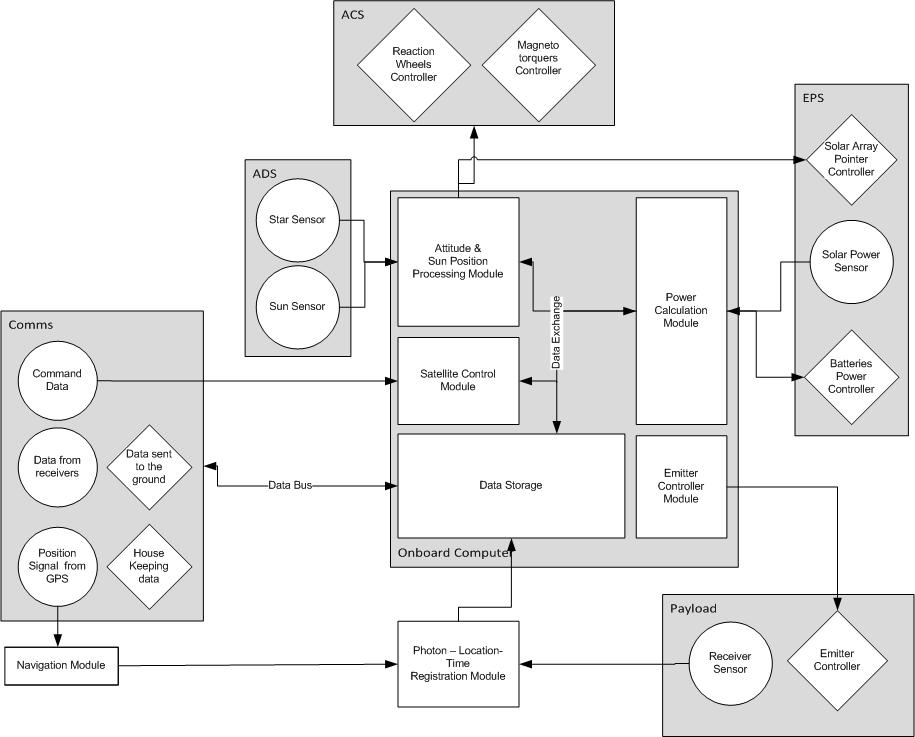
\includegraphics[width=1\textheight]{chapters/img/SWBDemit.jpg}
\caption{Software block diagram for emitter }
\label{fig:SWBDemit}
\end{figure}
\end{landscape}

\begin{landscape}
\begin{figure}[ht!]
\centering
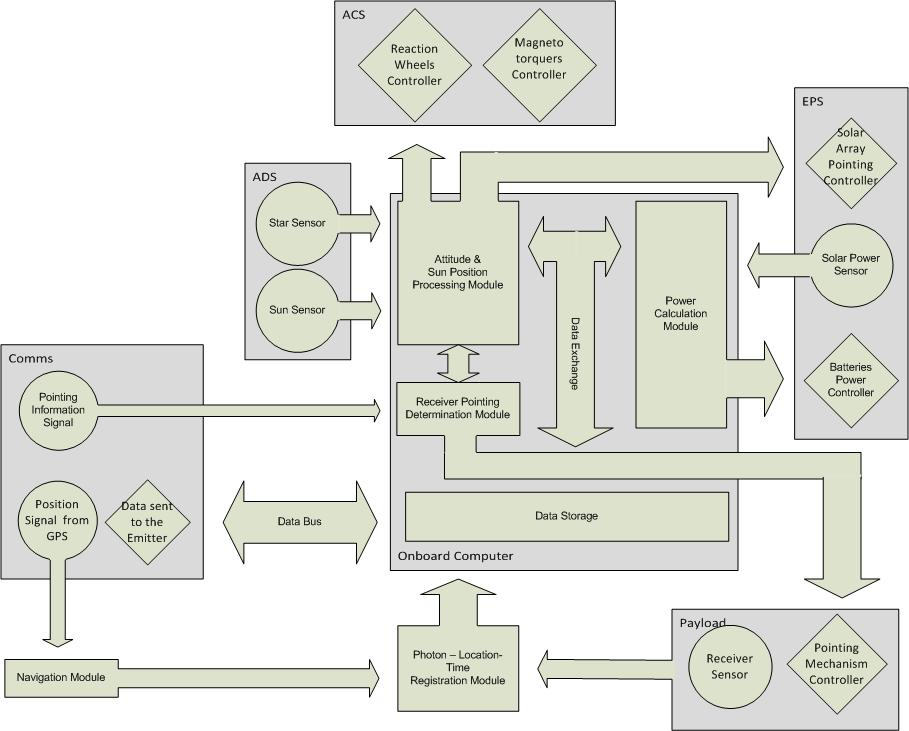
\includegraphics[width=1\textheight]{chapters/img/SWBDrec.jpg}
\caption{Software block diagram for receiver}
\label{fig:SWBDrec}
\end{figure}
\end{landscape}